\section{Introduction}
\label{sec:introduction}
% questioning the how

% Rise of DL
In recent years, deep learning models have demonstrated superior performance on a variety of tasks \cite{ruede2020multi, brinker2019deep, nguyen2020super}. While performance is still increasing and more tasks are being handled, their performance comes at the cost of complexity: models often use millions to billions of parameters to achieve universal function approximation.
This complexity means that they remain black boxes that cannot be interpreted even by experts.

% rise of XAI
Such a black box is able to predict well for unseen yet similar data, answering the question of \textit{what} is the most likely label for an input sample. 
However, most models will provide no answer to \textit{why} or \textit{how} the model chose this label for the instance and which features of the instance were crucial for making this prediction. 

For example, if a machine learning model is tasked with classifying images of cats (as in \autoref{fig:bb}), one would like to assume that the presence (or absence) of a cat in an image is indicative (contraindicative) of the classification of the image into the "cat" ("not cat") category.

\begin{figure}[t]
    \centering
    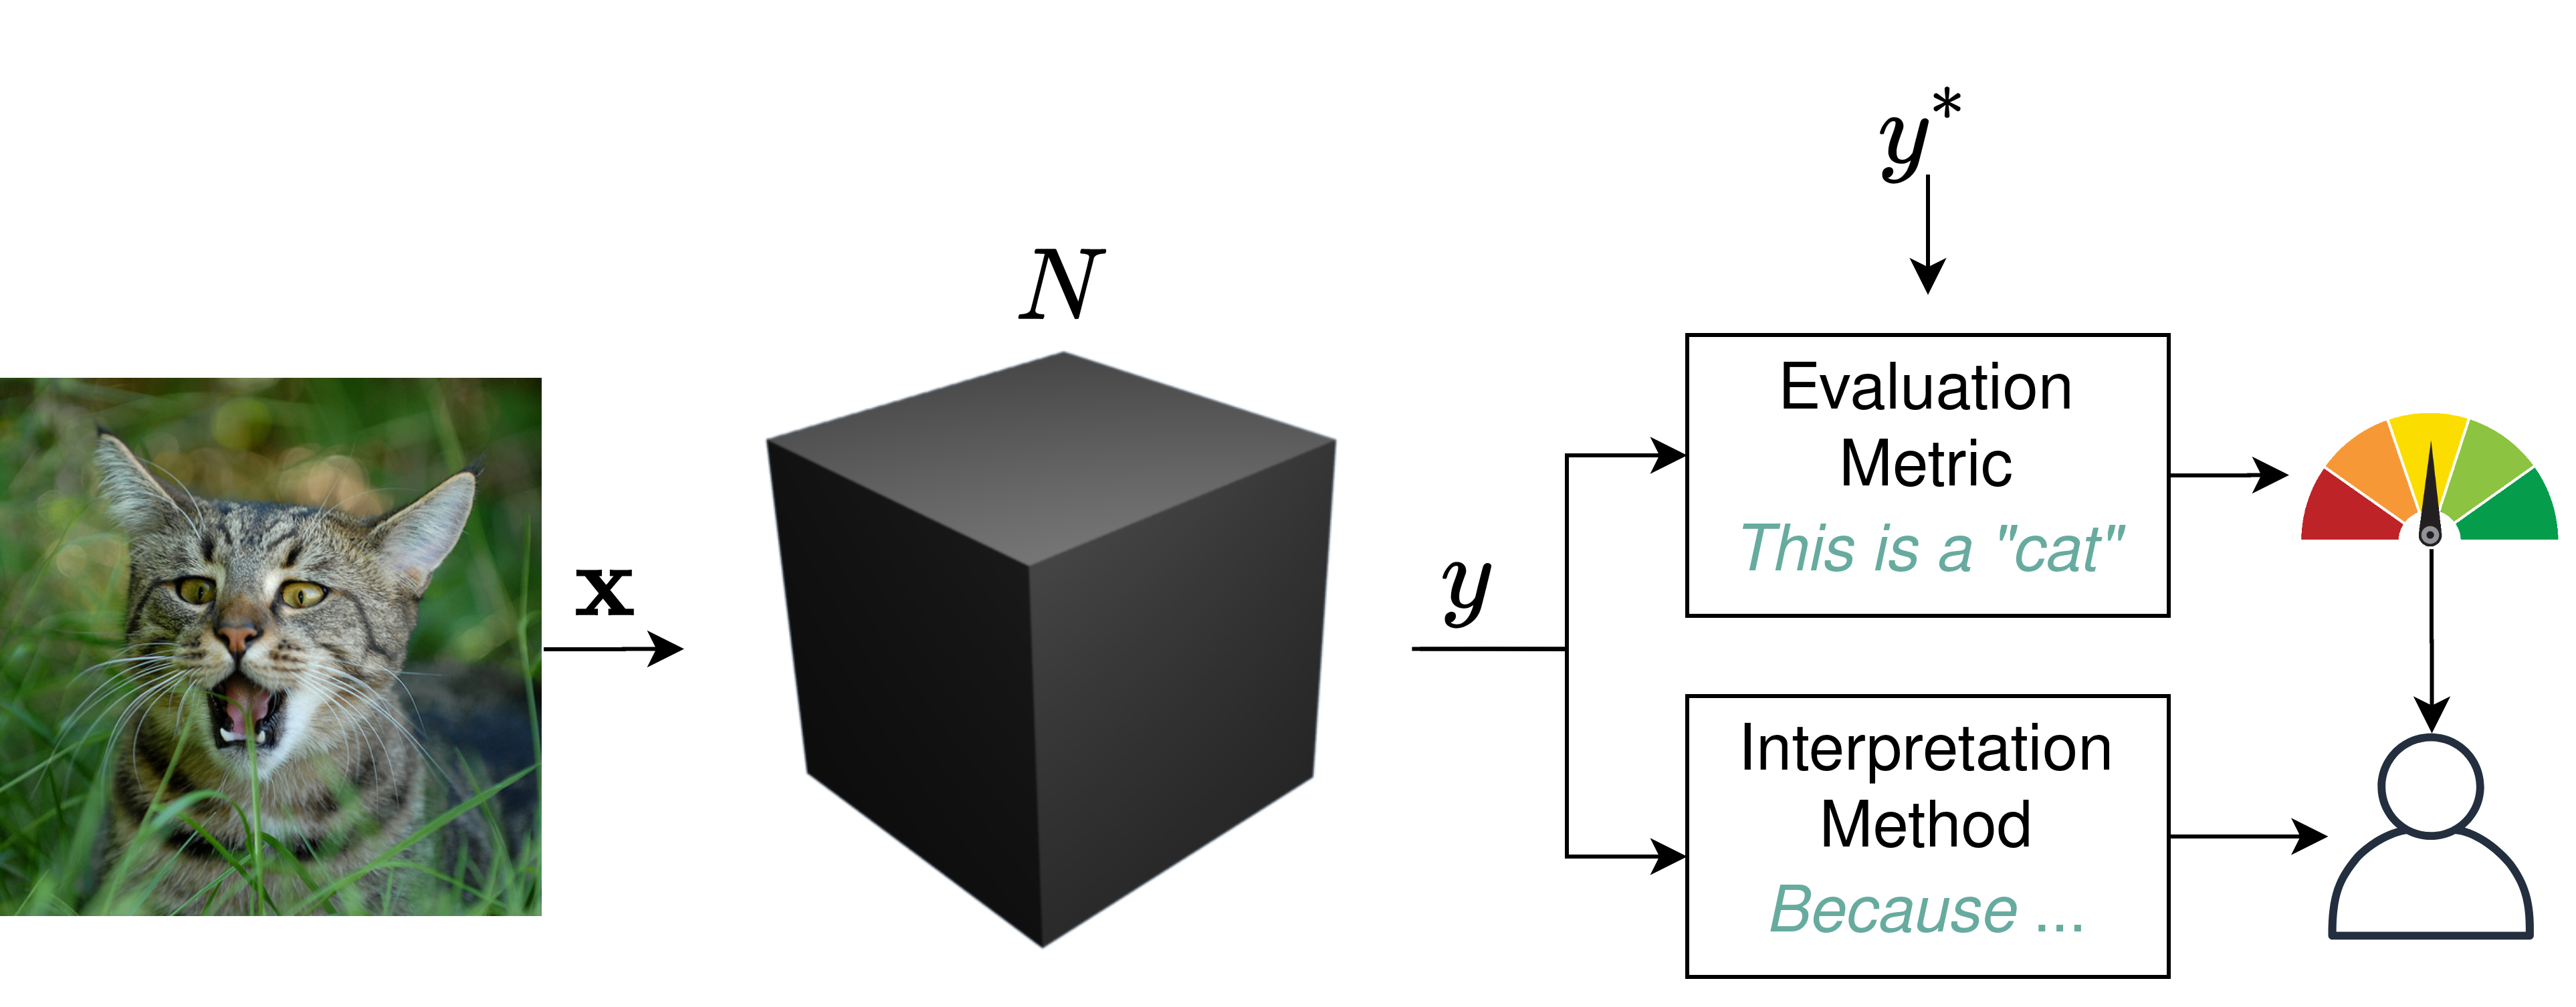
\includegraphics[width=\linewidth]{figures/bb_cat.png}
    \caption{Prediction pipeline using a machine learning model, depicted as blach box. Typically, evaluation metrics require the prediction $y$ and the ground truth label $y^*$ allowing for the assessmant of the model's accuracy. Additionally answering the question \textit{why}, i.e. making the model interpretable for a human, requires additional methods.}
    \label{fig:bb}
    \vspace{-0.3cm}
\end{figure}

Suppose a deep neural network predicts the risk for cancer from a mammogram, which is an image of breast tissue. A doctor would only use the algorithm if there is a way to validate that (1) tha algorithm is accurate (which can be measured in terms of the predictive accuracy), and (2) if the model is also using the correct indications in the data for predicting the risk of cancer. (1) is the standard approach for validating the performance of machine learning models, but in this example, one can clearly see why predictive accuracy might not be enough in many areas. For approaching (2), i.e. uncovering \textit{why} a model predicts a low / high risk of cancer, the research field of explainable artificial intelligence (XAI) offers a growing number of methods. Some research even suggests to allow 'peeking inside the black box' of deep learning models \cite{adadi2018peeking}.  

Automated algorithms are already in use in critical areas, such as medicine, chemistry, the criminal justice system, the financial sector or the piloting of self-driving cars \cite{chouldechova2017fair, elshawi2019interpretability, whitmore2016mapping}. % med, med, chemistry
Thus, as machine learning models are moving out of the lab into the real-world, the inability of humans to understand these (black box) models seems even more problematic. Not knowing how a model makes predictions, and not being able to detect systematic biases in the model, prevents the vastly advancing technology of machine learning from being used in highly sensitive and safety-critical applications.  

% TODO add security example?
Furthermore, the rise in machine learning model deployments also caused the development of adversarial attacks. These attacks attempt to fool a machine learning model by providing deceptive input. Fooling refers to the resulting malfunction of the model. 
% TODO first example
% hidden model and adversarial examples??

%%%%% iai
Not knowing about attacks and data arranged to exploit specific vulnerabilities has contributed to the field of XAI comprising topics of (1) \textit{model interpretations}, (2) \textit{adversarial attacks}, or manipulation methods and (3) the field of \textit{adversarial manipulations of model interpretations}. All these subfields have the common goal to make models more robust and safe for deployment. 
(1) refers to the development of techniques that can be used to understand and explain the decision making process of a machine learning model or even the development of models that are inherently interpretable. (2) is the field of detecting vulnerabilities in models that cause models to be deceived by altered input. 
(3) is the main topic of this paper, i.e. how to fool interpretation methods in order to detect vulnerabilities and malfunctions in interpretation methods. 
%%%% 
Ideally, an interpretation, or explanation method should indicate which pixels in the original image contribute to the prediction and also to what extent each pixel contributes. The extent to which each pixel contributes to a prediction is often called the \textit{importance} score of a feature. 
\autoref{fig:cat_lrp} shows the importance map built by an explanation method for the deep neural network.

\autoref{fig:lrp_cat} shows such a feature importance map produced by the interpretation method LRP \cite{bach2015pixel} applied to the neural network model Inception-v3 \cite{szegedy2016rethinking}. The input image is from the ImageNet dataset \cite{ILSVRC15}. As can be seen, the output of the interpretation method is projected onto the original image for better readability by humans. This importance map suggests that specific portions of the original cat image are important for the neural network make the high-confidence prediction (see..) of the category 'tiger cat'. 

\begin{figure}[ht]
    \centering
    \begin{subfigure}{0.48\linewidth}
      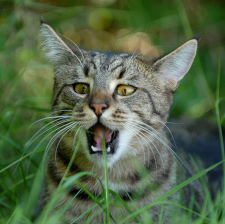
\includegraphics[width=\linewidth]{figures/cat.JPEG}
      \caption{Original.}
      \label{fig:lrp_cat_orig}
    \end{subfigure}
    \begin{subfigure}{0.48\linewidth}
      
\includegraphics[width=\linewidth]{figures/lrp_cat_heatmap.png}
      \caption{Feature importance map.}
      \label{fig:lrp_cat_lrp}
    \end{subfigure}
    \begin{subfigure}{0.8\linewidth}
        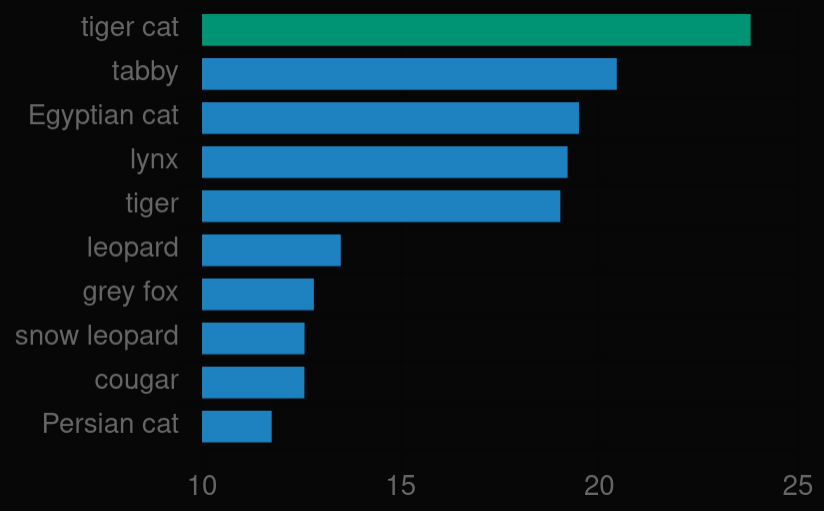
\includegraphics[width=\linewidth]{figures/cat_classification.png}
        \caption{Predictive accuracy.}
        \label{fig:cat_classification}
    \end{subfigure}
    \caption{Visualization of the feature importance map produced py the LRP interpreter applied to the image of a cat and an image classification model.}\label{fig:lrp_cat}
    \vspace{-0.3cm}
\end{figure}

%%%% 
% Thus, automated interpretation methods are required to make sense of the reasoning process and robustness of such deep learning based models and to ensure that a model makes decisions without unfair or hidden biases. 

% ethical examples: decisions where it is most crucial to have working systems

% https://towardsdatascience.com/interpretability-in-machine-learning-70c30694a05f 
% biases in ml models - boils down to data


% https://dl.acm.org/doi/pdf/10.1145/3387514.3405859?casa_token=lCc16GOTZsEAAAAA:gypLNU1o2Wwl3wt_b8stRbb0mgxEomX8PWprPeciNdkhVften3-5E01RM50e0W9NGQaGd4TrLOhA

While interpretation methods are already used for analysis of computer vision systems \cite{bach2015pixel, simonyan2013deep, zeiler2014visualizing}, text and sequence analysis \cite{ancona2017towards, arras2017relevant}, and deep learning in security \cite{evaluating_explanations_security}, there is still a lack in the the understanding of model interpretation methods. 

In particular, it is unclear how the variety of proposed model interpretation methods are related and what common concepts can be used to evaluate and compare them. 
Many works are dedicated to establish a formal definition of what it means to be interpretable, and how to select, evaluate and compare methods for generating explanations of machine learning models. \cite{murdoch2019definitions, lipton2018mythos}.



% While most of the approaches to explainability focus on the application to computer vision tasks, other domains are seldomly chosen. 

% todo cite a lot here
% https://www.bmc.com/blogs/machine-learning-interpretability-vs-explainability/ 7

% Visually appealing methods and easiy visual assessment of results. 
Most works in the field of XAI focus on image classification tasks, mostly because visualizations of a neural networks prediction can be easily verified by a human. The general purpose of image classification is to detect what objects are in an image. If a model works can be checked rather easily (if an image contains a cat, the prediction of a neural network should be cat and not some other object category). However, how it works (\textit{interpretability}), i.e. based on which features in the image the decision is made or which parameters in the model influence the prediction most, is an entirely different matter (\textit{explainability}).  

More importantly, while a big motivation for the development of robust and explainable systems is to overcome biases in models, datasets with direct implication of biases are seldomly used and by far not treated as benchmarking scenarios for explainability analyses.  


% Theoretical background
% why do adv attacks make sense? most models are trained on iid samples and thus not directly applicable to the real world, as the real world violates this statistical assumption. 



%%%%%%%%%%%%%%%%%%%%%%%% Outline
This article examines a topic at the intersection of explainable and adversarial machine learning research. 
The overview presented in this article examines the existing literature and contributions in the field of XAI focusing on methods to manipulate explanation methods.  
The critical literature analysis might serve as a motivation and step towards the biggest problems in XAI: How to make sure that interpretations of models are truly valid. 
This paper is structured as follows.

% TODO 
\autoref{sec:interpretation_methods} introduces common interpretation methods for machine learning models, and offers a taxonomy of the variety of techniques and a brief outline of popular interpretation methods.
In \autoref{sec:manipulation_methods}, the main topic of this paper, namely manipulation methods for deceiving interpretive techniques, is outlined. A taxonomy of methods is proposed and possible evaluation criteria are listed.

\autoref{sec:manipulations} provides a detailed review of important studies in the field of manipulation methods. The implacations of the current state-of-the-art in axplainable AI are discussed in section \autoref{sec:discussion}.